\documentclass{standalone} %tipo de documento "imagens solo"

\usepackage{tikz} %para imagens e gráficos vetoriais

\usepackage{circuitikz} %para desenhar circuitos elétricos

\usepackage{tkz-euclide} %define pontos no plano cartesiano

\usepackage{xcolor} %utilização de cores para estilos específicos 

\begin{document}

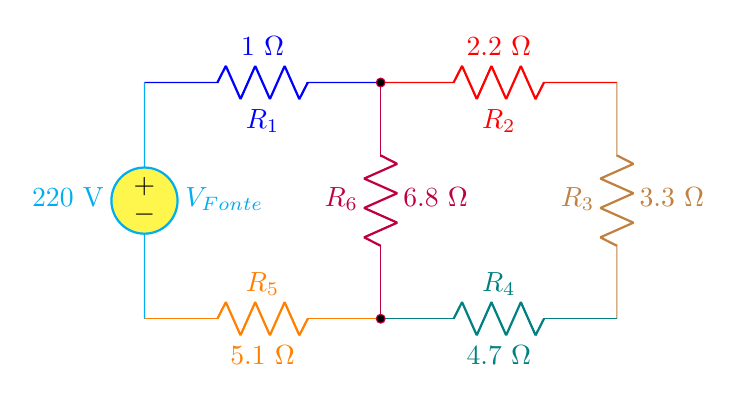
\begin{tikzpicture}[american] %define a tipologia dos componentes do circuito

%O comando \tkzDefPoints define os pontos no plano cartesiano para facilitar o posicionamento dos componentes do circuito. Os pontos são definidos pelas coordenadas (x/y/NomedoPonto)
\tkzDefPoints{
-9/5/A,
-6/5/B,
-3/5/C,
-3/2/D,
-6/2/E,
-9/2/F}

%Do ponto (-9,5) ao ponto (-6,5) cria um segmento com um resistor (R) no centro. Teste o comando "a" e "l" para incluir o rótulo do resistor, dentro ou fora do elemento. Desenha o elemento inteiro de azul forte. 
%---------------------------------------------------
\draw[blue] (A) to [R, a=$R_{1}$, l=$1$ $\Omega$] (B);
%---------------------------------------------------

%Do ponto (-6,5) ao ponto (-3,5) cria um segmento com um resistor (R) no centro. Teste o comando "a" e "l" para incluir o rótulo do resistor, dentro ou fora do elemento. Desenha o elemento inteiro de vermelho.
%---------------------------------------------------
\draw[red] (B) to [R, a=$R_{2}$, l=$2.2$ $\Omega$] (C);
%---------------------------------------------------

%Do ponto (-3,5) ao ponto (-3,2) cria um segmento com um resistor (R) no centro. Teste o comando "a" e "l" para incluir o rótulo do resistor, dentro ou fora do elemento. Desenha o elemento inteiro de marrom. 
%---------------------------------------------------
\draw[brown] (C) to [R, a=$R_{3}$, l=$3.3$ $\Omega$] (D);
%---------------------------------------------------

%Do ponto (-3,2) ao ponto (-6,2) cria um segmento com um resistor (R) no centro. Teste o comando "a" e "l" para incluir o rótulo do resistor, dentro ou fora do elemento. Desenha o elemento inteiro de verde-azulado.
%---------------------------------------------------
\draw[teal] (D) to [R, a=$R_{4}$, l=$4.7$ $\Omega$] (E);
%---------------------------------------------------

%Do ponto (-6,2) ao ponto (-9,2) cria um segmento com um resistor (R) no centro. Teste o comando "a" e "l" para incluir o rótulo do resistor, dentro ou fora do elemento. Desenha o elemento inteiro de laranja. 
%---------------------------------------------------
\draw[orange] (E) to [R, a=$R_{5}$, l=$5.1$ $\Omega$] (F);
%---------------------------------------------------


%Do ponto (-6,5) ao ponto (-6,2) cria um segmento com um resistor (R) no centro. Teste o comando "a" e "l" para incluir o rótulo do resistor, dentro ou fora do elemento. *-* inseri os nós no elemento. Desenha o elemento inteiro de roxo.
%-----------------------------------------
\draw[purple] (B) to [R, a=$R_{6}$, l=$6.8$ $\Omega$, *-*] (E);




%Do ponto (-9,2) ao ponto (-9,5) cria um segmento com uma fonte de tensão (vsource) no centro. Teste o comando "a" e "l" para incluir o rótulo do resistor, dentro ou fora do elemento. Desenha o elemento inteiro em ciano e preenche com a cor amarela em 70 %, com exceção do sinal de mais e menos (preto). 
%---------------------------------------------------
\draw[cyan, fill=yellow!70] (F) to [vsource, a=$V_{Fonte}$, l=$220$ V, invert] (A);
%---------------------------------------------------

\end{tikzpicture}

\end{document}
